In Figure \ref{fig:plot:binned-error-margins}, divergences greater than 5\% and lesser than -15\% were obtained with only 9.2\% of the dataset. With this in consideration, the process described in Section \ref{sec:Appendix:NarrowedEnergyPredictionErrorMarginRange:PreservingOutliers} was repeated without the data points responsible for the divergence outliers. This further narrowed down the error margin range to -11\%/+5\% by applying solar array dust factor adjustment of 5.4\% coupled with shadowing and other losses of 5\%. The resulting adjusted divergences are presented in Figure \ref{fig:plot:mer-energy-prediction-divergences-adjusted-without-outliers}:

\begin{figure}[h]
  \centering
  \hypersetup{linkcolor=captionTextColor}
  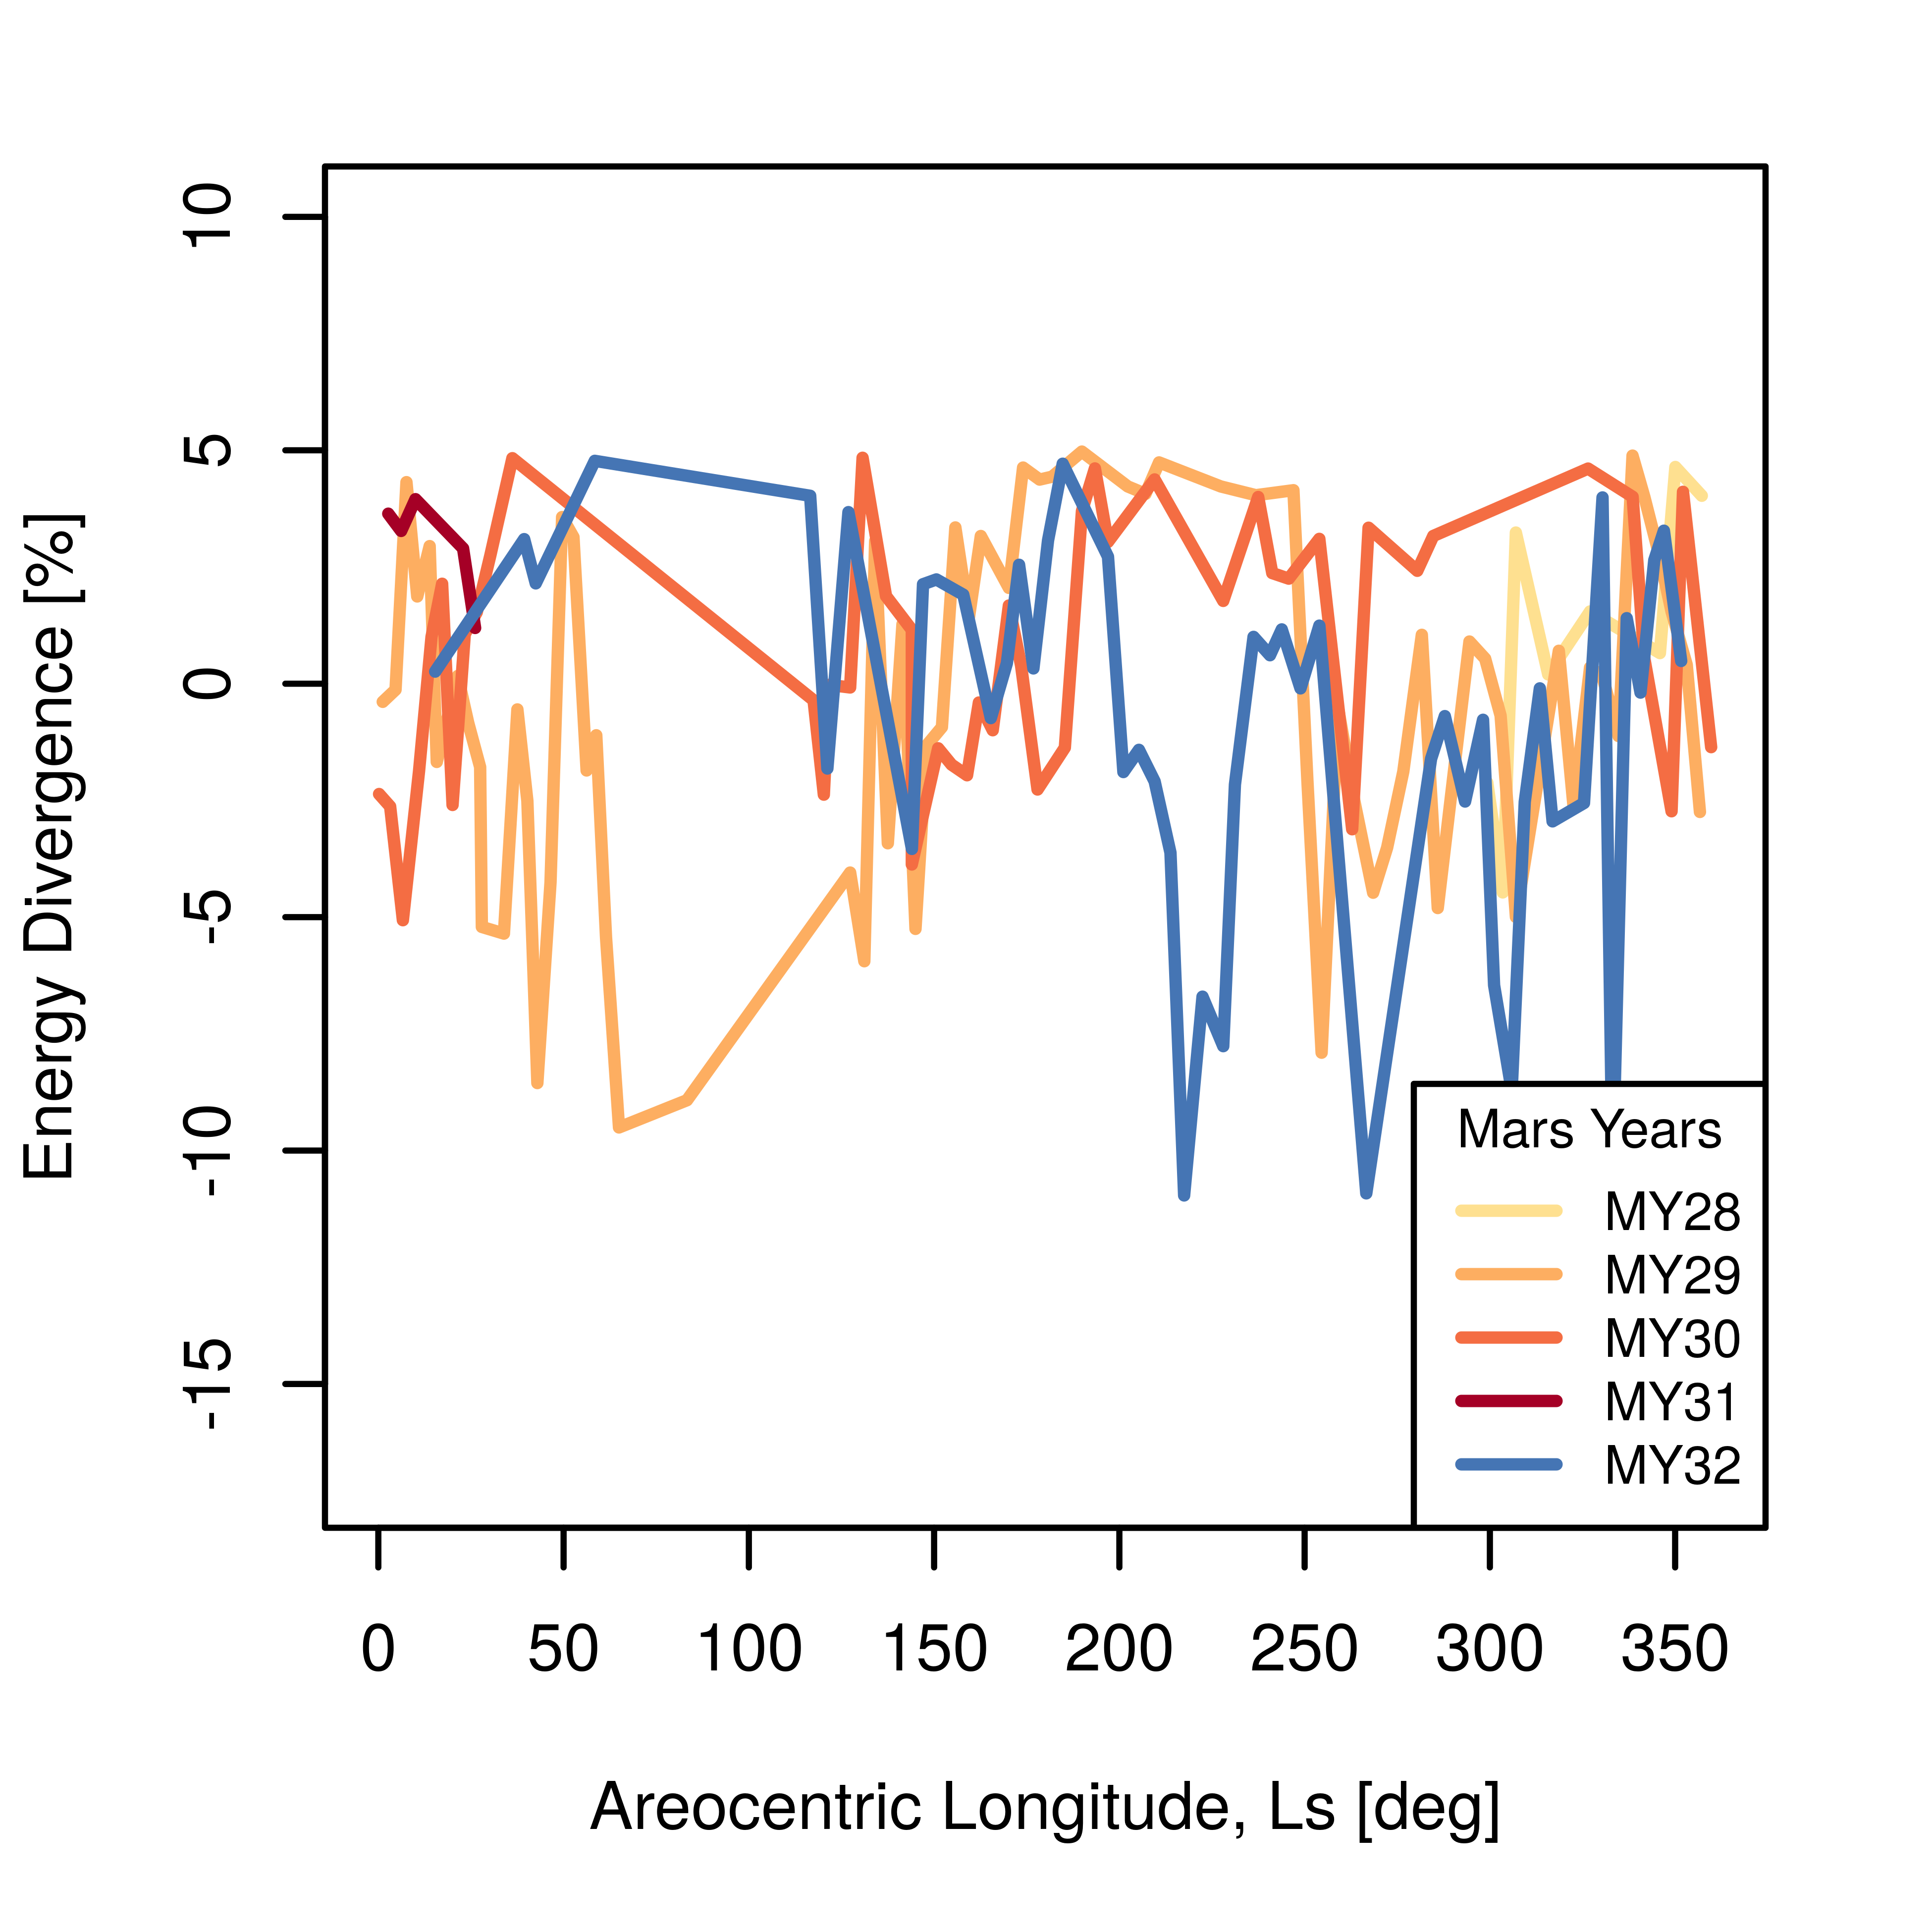
\includegraphics[width=0.8\linewidth]{sections/appendix/B/plots/energy-prediction-divergences-from-my28-to-my32-adjusted-without-outliers.png}\\
  \caption[Adjusted Outlierless divergences from measured MER Opportunity PV energy production]
          {Adjusted Outlierless divergences from measured MER Opportunity PV energy production.}
  \label{fig:plot:mer-energy-prediction-divergences-adjusted-without-outliers}
\end{figure}
